\chapter{Plan de Trabajo y Presupuesto}
\label{cap:plan_trabajo_presupuesto}

En este capítulo se formaliza la planificación temporal, la metodología de gestión, la estructura organizativa y el presupuesto económico del Trabajo de Fin de Máster. Atendiendo de forma rigurosa a las directrices de evaluación académica y al dictamen del tribunal evaluador, se presenta una descomposición detallada y coherente del proyecto estructurada en 200 horas de dedicación efectiva individual, ejecutadas en el periodo comprendido entre febrero y agosto (con una pausa total de actividad durante el mes de julio). Asimismo, se clarifica de manera inequívoca la naturaleza 100\% unipersonal de la autoría y el rol puramente metodológico de los perfiles funcionales simulados, estableciendo una gobernanza transparente y reproducible.

% ==============================================================================
% 4.1. METODOLOGÍA Y ESTRUCTURA DE DESCOMPOSICIÓN DEL TRABAJO (EDT)
% ==============================================================================
\section{Fases del Proyecto y Metodología}
\label{sec:fases_metodologia}

\subsection{Enfoque Metodológico}
\label{subsec:enfoque_metodologico}

Dada la naturaleza híbrida de la investigación ---que articula investigación teórica en física cuántica, ingeniería de software en compilación de circuitos y modelización financiera cuantitativa--- se ha adoptado una metodología ágil adaptada a proyectos de I+D computacional. El flujo de trabajo se organizó en iteraciones bisemanales (\textit{sprints}) orientadas a la obtención de incrementos funcionales verificables:
\begin{itemize}
    \item Al cierre de cada ciclo, se ejecutaron baterías de pruebas unitarias automatizadas (\texttt{pytest}) para certificar la equivalencia analítica de las matrices de coste antes de escalar a simulaciones de mayor dimensionalidad.
    \item La integración continua y el control de versiones se gestionaron íntegramente mediante Git y un repositorio privado alojado en GitHub, asegurando la trazabilidad de cada módulo del código fuente y de los manuscritos en \LaTeX.
\end{itemize}

\subsection{Estructura de Descomposición del Trabajo (EDT/WBS)}
\label{subsec:edt_wbs}

Para garantizar un control exhaustivo del alcance y permitir una asignación horaria transparente, el proyecto se ha estructurado en cinco Paquetes de Trabajo (\textit{Work Packages}, WP) secuenciales e interdependientes, desglosados en tareas elementales de nivel operativo:

\begin{enumerate}[leftmargin=*]
    \item \textbf{WP1: Gestión y Revisión Bibliográfica (20 horas)}
    \begin{itemize}
        \item \textit{T1.1. Revisión del estado del arte en QAOA y computación NISQ (12 h):} Análisis crítico de la literatura sobre algoritmos variacionales, mesetas estériles (\textit{Barren Plateaus}), Hamiltonianos de Ising y preservación de simetría.
        \item \textit{T1.2. Delimitación y modelado del problema financiero (8 h):} Formalización del problema de selección de carteras de Markowitz con restricción dura de cardinalidad exacta $K$ y análisis de su complejidad combinatoria NP-hard.
    \end{itemize}

    \item \textbf{WP2: Modelado Matemático y Formulación (30 horas)}
    \begin{itemize}
        \item \textit{T2.1. Construcción del modelo QUBO y calibración de penalizaciones (14 h):} Mapeo algebraico de la función objetivo y deducción analítica del multiplicador de penalización de Lagrange $P$ para la formulación penalizada estándar.
        \item \textit{T2.2. Derivación del Hamiltoniano de Ising y subespacio de Dicke (16 h):} Transformación afín de variables binarias a operadores de espín de Pauli $Z_i$, acoplamientos $J_{ij}$, campos locales $h_i$ y demostración analítica de la conmutación del operador XY-Mixer $[H_M^{XY}, \hat{K}] = 0$.
    \end{itemize}

    \item \textbf{WP3: Desarrollo de Software e Implementación del Algoritmo (65 horas)}
    \begin{itemize}
        \item \textit{T3.1. Pipeline de datos de mercado y preprocesado financiero (10 h):} Implementación de la ingesta automatizada desde Yahoo Finance, cálculo de retornos logarítmicos continuos, matrices de covarianza anualizadas y división temporal \textit{In-Sample} / \textit{Out-of-Sample}.
        \item \textit{T3.2. Implementación de estados de Dicke y transpilación del XY-Mixer (22 h):} Programación en el framework \texttt{Qrisp} del circuito determinista de preparación del estado de Dicke $|D_K^N\rangle$ y síntesis del mezclador $XY$ sobre topología de acoplamiento lineal y en anillo.
        \item \textit{T3.3. Esquema de regularización bicapa TQA y Ridge $L_2$ (18 h):} Desarrollo de la clase \texttt{RegularizedQAOAProblem} para calcular ángulos de inicio adiabáticos (TQA) e integrar la penalización continua cuadrática en el optimizador clásico COBYLA.
        \item \textit{T3.4. Integración de solvers clásicos de referencia (15 h):} Implementación de la interfaz con Gurobi Optimizer (\textit{Branch-and-Bound}) y Simulated Annealing (\texttt{dwave-neal}), y creación de la suite de tests unitarios (\texttt{tests/}).
    \end{itemize}

    \item \textbf{WP4: Experimentación, Simulación y Benchmarking (35 horas)}
    \begin{itemize}
        \item \textit{T4.1. Ejecución de simulaciones variacionales (18 h):} Ejecución de las 40 instancias parametrizadas en escalado dimensional ($N \in [6, 20]$ cúbits) y barrido de profundidad del ansatz ($p \in [1, 10]$).
        \item \textit{T4.2. Recopilación de métricas y evaluación comparativa (17 h):} Procesamiento de los datos de convergencia, cálculo del Optimization GAP, tasa de factibilidad matemática, Ratio de Sharpe OOS y análisis del coste temporal en CPU.
    \end{itemize}

    \item \textbf{WP5: Redacción de la Memoria y Diseminación (50 horas)}
    \begin{itemize}
        \item \textit{T5.1. Estructuración y redacción técnica de capítulos en \LaTeX\ (32 h):} Redacción exhaustiva y rigurosa de la memoria técnica conforme a los estándares académicos del máster y el feedback del tribunal.
        \item \textit{T5.2. Generación automatizada de gráficos vectoriales y tablas (10 h):} Desarrollo de scripts en Python (\texttt{matplotlib}/\texttt{seaborn}) para la renderización de figuras analíticas en alta resolución (300 DPI) y cuadros comparativos.
        \item \textit{T5.3. Control de calidad, revisión ortotipográfica y defensa oral (8 h):} Verificación de coherencia metodológica entre objetivos y conclusiones, maquetación final y elaboración del soporte visual para la defensa.
    \end{itemize}
\end{enumerate}

La Figura~\ref{fig:wbs_tree} ilustra la disposición jerárquica de la Estructura de Descomposición del Trabajo descrita.

\begin{figure}[htbp]
    \centering
    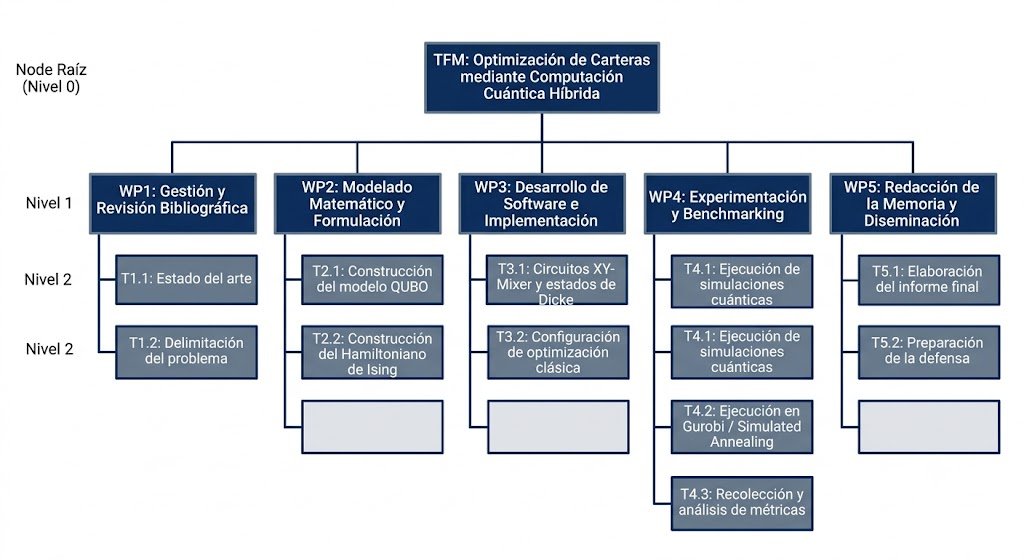
\includegraphics[width=0.95\textwidth]{output/figures_tfm/4.PlanTrabajo/wbs_tree.jpg}
    \caption{Estructura de Descomposición del Trabajo (EDT/WBS) del proyecto de investigación.}
    \label{fig:wbs_tree}
\end{figure}

% ==============================================================================
% 4.2. PLANIFICACIÓN TEMPORAL Y CRONOGRAMA
% ==============================================================================
\section{Planificación Temporal y Calendario}
\label{sec:planificacion_temporal}

\subsection{Cronograma de Ejecución e Hitos}
\label{subsec:cronograma_hitos}

El proyecto se planificó para un periodo global de siete meses naturales (febrero a agosto), distribuyendo el esfuerzo en 200 horas efectivas de trabajo. Con el fin de reflejar con total veracidad el avance real del proyecto, se documenta que durante el mes de julio la actividad computacional y de redacción estuvo completamente pausada (0 horas imputadas), concentrándose el esfuerzo de experimentación final, redacción avanzada y consolidación de la memoria en los meses de mayo, junio y agosto.

Para evaluar de forma cuantitativa el avance, se establecieron cinco hitos de control (\textit{Milestones}):
\begin{itemize}
    \item \textbf{M1 (Final de febrero):} Estado del arte consolidado y delimitación formal del problema de cardinalidad en carteras.
    \item \textbf{M2 (Final de marzo):} Formulación analítica QUBO/Ising y verificación algebraica del operador XY-Mixer.
    \item \textbf{M3 (Final de abril):} Repositorio de software plenamente operativo y validado con tests unitarios.
    \item \textbf{M4 (Mediados de junio):} Campaña experimental completada y dataset consolidado en \texttt{results.csv}.
    \item \textbf{M5 (Final de agosto):} Memoria técnica completa depositada y presentación oficial para la convocatoria extraordinaria.
\end{itemize}

El cronograma temporal detallado y la distribución de los paquetes de trabajo se representan en el diagrama de Gantt de la Figura~\ref{fig:gantt_chart}.

\begin{figure}[htbp]
    \centering
    \includegraphics[width=0.98\textwidth]{output/figures_tfm/4.PlanTrabajo/gantt_chart2.png}
    \caption{Diagrama de Gantt del proyecto (febrero--agosto, con pausa en julio y 200 h de dedicación total).}
    \label{fig:gantt_chart}
\end{figure}

\subsection{Determinación del Camino Crítico}
\label{subsec:camino_critico}

El análisis de dependencias técnicas revela que el camino crítico del proyecto está conformado por la secuencia lineal:
\begin{equation}
    \text{WP2 (Modelado Matemático)} \longrightarrow \text{WP3 (Desarrollo de Software)} \longrightarrow \text{WP4 (Experimentación)} \longrightarrow \text{WP5 (Redacción Final)}
\end{equation}
Cualquier desviación o retraso en la derivación de los operadores cuánticos o en la transpilación del estado de Dicke en \texttt{Qrisp} impacta de forma directa e inmediata en la campaña de benchmarking en CPU y en la posterior redacción de los resultados empíricos, al no existir holgura temporal en la cadena de desarrollo nuclear.

% ==============================================================================
% 4.3. ESTRUCTURA ORGANIZATIVA Y GESTIÓN DE RECURSOS HUMANOS
% ==============================================================================
\section{Estructura Organizativa y Aclaración de Recursos Humanos}
\label{sec:organizacion_rrhh}

\subsection{Declaración de Autoría Individual y Roles Funcionales}
\label{subsec:autoria_roles}

En respuesta directa al requerimiento del tribunal evaluador relativo a la clarificación de los recursos humanos, se declara de manera explícita y formal lo siguiente:

\begin{quote}
\textit{El presente Trabajo de Fin de Máster ha sido realizado de forma \textbf{estrictamente individual y unipersonal} por el autor, \textbf{Aimar Etxaniz Urbieta}, quien ha asumido la totalidad del diseño matemático, programación del software, ejecución de las simulaciones, análisis de datos y redacción de la memoria.}
\end{quote}

La referencia presente en versiones preliminares a dos perfiles técnicos especializados (\textit{Quantum Computing Engineer} y \textit{Quantitative Financial Analyst}) responde exclusivamente a una \textbf{simulación de roles funcionales e interdisciplinares} habituales en la industria de las tecnologías financieras cuánticas (\textit{Quantum Fintech}). Esta subdivisión conceptual se empleó con fines metodológicos para estructurar los dos grandes dominios de conocimiento requeridos por el proyecto:
\begin{enumerate}
    \item \textbf{Rol de Ingeniería Cuántica (\textit{Quantum Engineer}):} Cubre el diseño físico de circuitos cuánticos, transpilación del XY-Mixer, cálculo de anclas TQA y desarrollo del simulador en \texttt{Qrisp}.
    \item \textbf{Rol de Análisis Cuantitativo (\textit{Quant Analyst}):} Cubre la ingesta y depuración de series temporales de renta variable, calibración de covarianzas, sintonización del parámetro de aversión al riesgo $\lambda$ y cálculo de métricas financieras (\textit{Sharpe Ratio Out-of-Sample}).
\end{enumerate}

Ambas dimensiones fueron ejecutadas en su totalidad por el mismo y único autor, distribuyendo las 200 horas de dedicación total de manera equilibrada entre ambas áreas de competencia.

\subsection{Matriz de Responsabilidades y Desglose Horario Consolidado}
\label{subsec:desglose_horario_tabla}

El Cuadro~\ref{tab:desglose_horas_tareas} detalla la distribución exacta de las 200 horas de dedicación efectiva entre los cinco paquetes de trabajo y sus tareas asociadas, reflejando el peso preponderante asignado a la ingeniería de software (65 horas) y a la redacción rigurosa de la documentación (50 horas).

\begin{table}[htbp]
    \centering
    \small
    \caption{Desglose detallado de dedicación horaria por paquete de trabajo y tarea (Total: 200 h).}
    \label{tab:desglose_horas_tareas}
    \renewcommand{\arraystretch}{1.2}
    \begin{tabular}{p{2.2cm}p{7.8cm}r}
        \toprule
        \textbf{Paquete (WP)} & \textbf{Tarea Específica / Actividad} & \textbf{Dedicación (h)} \\
        \midrule
        \textbf{WP1: Revisión} & T1.1. Estado del arte en QAOA, Barren Plateaus y NISQ & 12 \\
        & T1.2. Delimitación y modelado de restricciones financieras & 8 \\
        \rowcolor{gray!10} \multicolumn{2}{l}{\textbf{Subtotal WP1}} & \textbf{20} \\
        \midrule
        \textbf{WP2: Modelado} & T2.1. Construcción del modelo QUBO y calibración de penalización $P$ & 14 \\
        & T2.2. Derivación analítica del Hamiltoniano de Ising y simetría XY & 16 \\
        \rowcolor{gray!10} \multicolumn{2}{l}{\textbf{Subtotal WP2}} & \textbf{30} \\
        \midrule
        \textbf{WP3: Software} & T3.1. Pipeline de descarga y preprocesado de datos de mercado & 10 \\
        & T3.2. Implementación de estados de Dicke y transpilador XY-Mixer en Qrisp & 22 \\
        & T3.3. Desarrollo del módulo de regularización bicapa TQA + Ridge $L_2$ & 18 \\
        & T3.4. Integración de solvers clásicos (Gurobi, SA) y tests unitarios & 15 \\
        \rowcolor{gray!10} \multicolumn{2}{l}{\textbf{Subtotal WP3 (Desarrollo de Código)}} & \textbf{65} \\
        \midrule
        \textbf{WP4: Experim.} & T4.1. Ejecución de campañas de simulación ($N=6..20$ cúbits, $p=1..10$) & 18 \\
        & T4.2. Análisis de métricas (GAP, Viabilidad, Sharpe OOS, Tiempos) & 17 \\
        \rowcolor{gray!10} \multicolumn{2}{l}{\textbf{Subtotal WP4}} & \textbf{35} \\
        \midrule
        \textbf{WP5: Memoria} & T5.1. Redacción técnica y estructuración de la memoria en \LaTeX & 32 \\
        & T5.2. Generación automatizada de gráficos vectoriales y cuadros & 10 \\
        & T5.3. Revisión ortotipográfica, control de calidad y preparación de defensa & 8 \\
        \rowcolor{gray!10} \multicolumn{2}{l}{\textbf{Subtotal WP5 (Documentación y Diseminación)}} & \textbf{50} \\
        \midrule
        \multicolumn{2}{l}{\textbf{TOTAL DEDICACIÓN EFECTIVA DEL PROYECTO}} & \textbf{200} \\
        \bottomrule
    \end{tabular}
\end{table}

% ==============================================================================
% 4.4. PRESUPUESTO DETALLADO Y PLAN DE FINANCIACIÓN
% ==============================================================================
\section{Presupuesto Detallado y Plan de Financiación}
\label{sec:presupuesto_financiacion}

\subsection{Costes Directos de Personal}
\label{subsec:costes_personal}

El presupuesto de recursos humanos se calcula computando las 200 horas efectivas de dedicación del autor bajo una tarifa profesional de mercado estándar para perfiles de ingeniería de software cuántico y análisis cuantitativo de 35~\euro/h. Esto consolida un coste directo de personal de:
\begin{equation}
    \text{Coste Personal} = 200\text{ horas} \times 35\text{ \euro/h} = 7.000\text{ \euro}
\end{equation}

\subsection{Costes de Infraestructura Cloud y Licencias de Software}
\label{subsec:costes_cloud_software}

\begin{itemize}
    \item \textbf{Cómputo Clásico Acelerado (Google Colab Pro / AWS EC2):} Aprovisionamiento de entornos con alta memoria RAM y núcleos de procesamiento dedicados para sostener las simulaciones densas de vectores de estado $2^N$ en instancias complejas ($N=18..20$). Coste imputado: 250~\euro.
    \item \textbf{Acceso a Entornos Cuánticos (AWS Braket / QPUs):} Coste de emulación de canales de ruido y pruebas de concepto en plataformas cloud. Coste estimado: 800~\euro.
    \item \textbf{Licencias de Software y Optimizadores:} Licencia académica/comercial prorrateada de Gurobi Optimizer para benchmarking determinista: 600~\euro.
    \item \textbf{Amortización de Hardware Local:} Amortización técnica de la estación de trabajo (ordenador personal con procesador Intel i7, 32 GB RAM) prorrateada para los 7 meses de uso del proyecto sobre una vida útil de 36 meses: 350~\euro.
\end{itemize}

\subsection{Presupuesto Consolidado}
\label{subsec:presupuesto_consolidado}

El Cuadro~\ref{tab:presupuesto_consolidado} consolida todas las partidas económicas del proyecto, incluyendo un margen de contingencia del 10\% para imprevistos operativos en computación en la nube, fijando el presupuesto global en 9.900~\euro\ (IVA excluido).

\begin{table}[htbp]
    \centering
    \small
    \caption{Presupuesto financiero consolidado del proyecto de investigación.}
    \label{tab:presupuesto_consolidado}
    \renewcommand{\arraystretch}{1.25}
    \begin{tabular}{p{3.2cm}p{6.5cm}r}
        \toprule
        \textbf{Categoría} & \textbf{Descripción de la Partida} & \textbf{Coste Total (\euro)} \\
        \midrule
        \textbf{Recursos Humanos} & Dedicación efectiva individual de ingeniería e investigación (200 h $\times$ 35 \euro/h) & 7.000 \\
        \textbf{Cómputo Cloud} & Servidores de alta memoria en AWS EC2 / Google Colab Pro & 250 \\
        \textbf{Plataformas Cuánticas} & Créditos de experimentación en la nube cuántica (AWS Braket) & 800 \\
        \textbf{Software \& Licencias} & Licencia prorrateada de Gurobi Optimizer API & 600 \\
        \textbf{Amortización HW} & Amortización de estación de trabajo local (7 meses prorrateados) & 350 \\
        \addlinespace
        \textbf{Subtotal Neto} & & \textbf{9.000} \\
        \textbf{Contingencias (10\%)} & Reserva operativa para sobrecostes de computación y red & 900 \\
        \midrule
        \textbf{TOTAL GENERAL} & \textbf{(Impuestos no incluidos)} & \textbf{9.900} \\
        \bottomrule
    \end{tabular}
\end{table}